\section{Theory} \label{sec:theory}

\subsection{Regression} \label{sec:regression}
A few general words about regression

\subsubsection{Ordinary Least Square (OLS)} \label{sec:OLS}
Suppose we have a set of points $\{(x_1, y_1), (x_2, y_2),\hdots, (x_n, y_n)\}$, and we want to fit a p'th order polynomial to them. The most intuitive way would be to find coefficients $\vec{\beta}$ which minimize the error in
\begin{align*}
y_1&=\beta_0x_1^0+\beta_1x_1^1+\hdots+\beta_px_1^p+\varepsilon_1\\
y_2&=\beta_0x_2^0+\beta_1x_2^1+\hdots+\beta_px_2^p+\varepsilon_2\\
\vdots\\
y_n&=\beta_0x_n^0+\beta_1x_n^1+\hdots+\beta_px_n^p+\varepsilon_n,
\end{align*}
which for OLS is defines as
\begin{equation}
\text{MSE}=\sum_i\varepsilon_i^2
\end{equation}
NEED TO REWRITE THIS + COST FUNCTION

Standard cost function

\begin{equation}
Q(\vec{\beta})=\sum_{i=0}^{n-1}(y_i-\tilde{y}_i)^2=(\vec{y}-\hat{X}\vec{\beta})^T(\vec{y}-\hat{X}\vec{\beta})
\end{equation}

Instead of dealing with a set of equations, we can apply linear algebra. One can easily see that the equations above correspond to
\begin{equation}
\vec{y}=\hat{X}^T\vec{\beta}+\vec{\varepsilon},
\label{eq:y_xb}
\end{equation}
with
\begin{equation}
\hat{X}=\begin{pmatrix}
x_1^0&x_1^1&x_1^2&\hdots&x_1^p\\
x_2^0&x_2^1&x_2^2&\hdots&x_2^p\\
\vdots&\vdots&\vdots&\ddots&\vdots\\
x_n^0&x_n^1&x_n^2&\hdots&x_n^p
\end{pmatrix}
\end{equation}
and
\begin{equation}
\vec{\beta}=(\beta_0, \beta_1, \hdots, \beta_p).
\end{equation}

For a nonsingular matrix $\hat{X}$ (but not necessary symmetric) we can find the optimal $\vec{\beta}$ by solving
\begin{equation}
\vec{\beta}=(\hat{X}^T\hat{X})^{-1}\hat{X}^T\vec{y},
\end{equation}
which again corresponds to minimizing the cost function,
\begin{equation}
\vec{\beta}=\text{argmin},\vec{\beta}\bigg\{\sum_{i=1}^{n}\Big(y_i-\beta_0-\sum_{j=1}^px_{ij}\beta_j\Big)^2\bigg\}.
\end{equation}

CONFIDENCE INTERVAL of $\hat{\beta}$: Var($\hat{\beta}$).

This works perfectly when all rows in $\hat{X}$ are linearly independent, but this will generally not be the case for large data sets. If we are not able to diagonalize the matrix, we will not be able to calculate $(\hat{X}^T\hat{X})^{-1}$, so we need to do something smart. 

Fortunately there is a simple trick we can do to make all matrices diagonalizable; we can add a diagonal matrix to the initial matrix. 


\subsubsection{Ridge regression} \label{sec:ridge}
Ridge regression is a widely used method that can handle singularities in matrices. The idea is to modify the standard cost function by adding a small term,
\begin{equation}
Q^{\text{ridge}}(\vec{\beta})=\sum_{i=1}^N(y_i-\tilde{y_i})^2+\lambda||\vec{\beta}||_2^2,
\end{equation}
where $\lambda$ is the so-called \textit{penalty} and $||\vec{v}||_2$ is defined as
\begin{equation}
||\vec{v}||_2=\sqrt{\vec{v}^T\vec{v}}=\Big(\sum_{i=1}^Nv_i^2\Big)^{1/2}.
\end{equation}
This will eliminate the singularity problem.

Further we find the optimal $\vec{\beta}$ values by minimizing the function 
\begin{equation}
\vec{\beta}^{\text{ridge}}=\text{argmin},\vec{\beta}\bigg\{\sum_{i=1}^{n}\Big(y_i-\beta_0-\sum_{j=1}^px_{ij}\beta_j\Big)^2+\lambda\sum_{j=1}^p\beta_j^2\bigg\}, 
\end{equation}
or we could simply solve the equation
\begin{equation}
\vec{\beta}^{\text{ridge}}=(\hat{X}^T\hat{X}+\lambda I)^{-1}\hat{X}^T\vec{\beta}.
\end{equation}
In the latter equation we can easily see why this solves our problem.

\subsubsection{Lasso regression} \label{sec:lasso}
The idea behind Lasso regression is similar to the idea behind Ridge regression, and they differ only by the exponent factor in the last term. The modified cost function now writes
\begin{equation}
Q^{\text{lasso}}(\vec{\beta})=\sum_{i=1}^N(y_i-\tilde{y_i})^2+\lambda||\vec{\beta}||_2,
\end{equation}
and to find the optimal coefficients $\vec{\beta}$, we need to minimize
\begin{equation}
\vec{\beta}^{\text{lasso}}=\text{argmin},\vec{\beta}\bigg\{\sum_{i=1}^{n}\Big(y_i-\beta_0-\sum_{j=1}^px_{ij}\beta_j\Big)^2+\lambda\sum_{j=1}^p\beta_j\bigg\}.
\end{equation}

\subsubsection{General form}
We can generalize the models above to a minimization problem where we have a $q$ in the last exponent, 
\begin{equation}
\vec{\beta}^q=\text{argmin},\vec{\beta}\bigg\{\sum_{i=1}^{n}\Big(y_i-\beta_0-\sum_{j=1}^px_{ij}\beta_j\Big)^2+\lambda\sum_{j=1}^p\beta_j^q\bigg\},
\end{equation}
such that $q=2$ corresponds to the Ridge method and $q=1$ is associated with Lasso regression. It can also be interesting to try other $q$-values.

\subsection{Higher order regression} \label{sec:higher_reg}
We can use the same approach as above when dealing with regression of higher order, since the problem is to fit a function to points, no matter how many components they have. We will first take a look at how we can fit a 2D polynomial to some terrain data, before we briefly describe how to fit a function of arbitrary order to points.

\subsubsection{Terrain} \label{sec:terrain}
A set of data points $\{(x_1, y_1, z_1), (x_2, y_2, z_2),\hdots, (x_n, y_n,z_n)\}$ gives some coordinates in space, which for instance can describe the terrain. The system of linear equations to solve can then be lined up as 
\begin{align*}
z_1&=\beta_0x_1^0y_1^0+\beta_1x_1^1y_1^0+\beta_2x_1^0y_1^1+\hdots+\beta_px_1^py_1^p+\varepsilon_1\\
z_2&=\beta_0x_2^0y_2^0+\beta_1x_2^1y_2^0+\beta_2x_2^0y_2^1+\hdots+\beta_px_2^py_2^p+\varepsilon_2\\
\vdots\\
z_n&=\beta_0x_n^0y_n^0+\beta_1x_n^1y_n^0+\beta_2x_n^0y_n^1+\hdots+\beta_px_n^py_n^p+\varepsilon_n,
\end{align*}
when fitting a polynomial of p'th order. In general the order associated with x-direction do not need to be the same as the order associated with y-direction. 

We can set up a similar equation as for the first order case, presented in equation \eqref{eq:y_xb}, but we will now (typically) have $\vec{z}$ on the left hand side and $\hat{X}$ will contain both x- and y-coordinates:
\begin{equation}
\vec{z}=\hat{X}^T\vec{\beta}.
\end{equation}
The coordinate matrix $\hat{X}$ will now looks like
\begin{equation}
\hat{X}=
\begin{pmatrix}
x_1^0y_1^0&x_1^1y_1^0&x_1^0y_1^1&x_1^1y_1^1&\hdots&x_1^py_1^p\\
x_2^0y_2^0&x_2^1y_2^0&x_2^0y_2^1&x_2^1y_2^1&\hdots&x_2^py_2^p\\
\vdots&\vdots&\vdots&\vdots&\ddots&\vdots\\
x_n^0y_n^0&x_n^1y_n^0&x_n^0y_n^1&x_n^1y_n^1&\hdots&x_n^py_n^p
\end{pmatrix}
\end{equation}
and we can again use the OLS method to find $\vec{\beta}$, i.e, calculating
\begin{equation}
\vec{\beta}=(\hat{X}^T\hat{X})^{-1}\hat{X}^T\vec{z}.
\end{equation}
Similarly we can use ridge and lasso regression in the same way as when fitting 1D polynomials. 

In this project one we will actually deal with terrain data. Firstly we implement some regression tools which fit a 2D function to points in space. To verify the implementation, we pick points from a known function such that we know the result. The specific verification function used is the Franke Function, which looks like

\begin{align*}
f(x,y) &= \frac{3}{4}\exp{\left(-\frac{(9x-2)^2}{4} - \frac{(9y-2)^2}{4}\right)}+\frac{3}{4}\exp{\left(-\frac{(9x+1)^2}{49}- \frac{(9y+1)}{10}\right)} \\
&+\frac{1}{2}\exp{\left(-\frac{(9x-7)^2}{4} - \frac{(9y-3)^2}{4}\right)} -\frac{1}{5}\exp{\left(-(9x-4)^2 - (9y-7)^2\right) },
\end{align*}
and is a smooth 2D function as one can see in figure \eqref{fig:franke}.

 \begin{figure} [H]
 	\centering
 	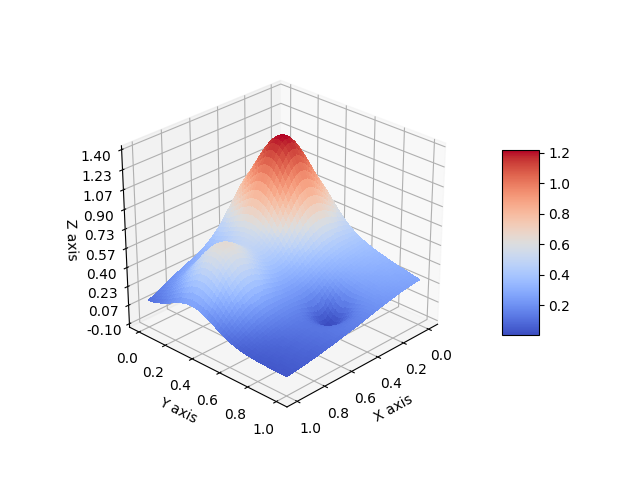
\includegraphics[scale=0.8]{../plots/franke.png}
 	\caption{The Franke function in the interval $x\in[0,1]$, $y\in[0,1]$, $z\in[0, 1.2]$.}
 	\label{fig:franke}
 \end{figure}

Secondly we use the verified regression tools to fit a polynomial to real terrain data.
NEED TO ADD A SENTENCE OR TWO HERE

\subsubsection{Higher order}
There should be no surprise that we can extend the theory above to even higher orders. 
Although we stick to 2D regression in this project, I add this section for completeness. 


\subsection{Error analysis}

Cost function (loss function) 

Different methods to estimate error:
\begin{itemize}
\item{Absolute error}
\item{Relative error}
\item{Mean square error (MSE)}
\item{R$^2$ score function}
\end{itemize}

